\section{Conclusiones}
\subsection{Respuestas}

\begin{frame}
    \frametitle{Preguntas investigadas}
    \begin{columns}
        \column{0.5\textwidth}
        \begin{figure}
            \begin{center}
                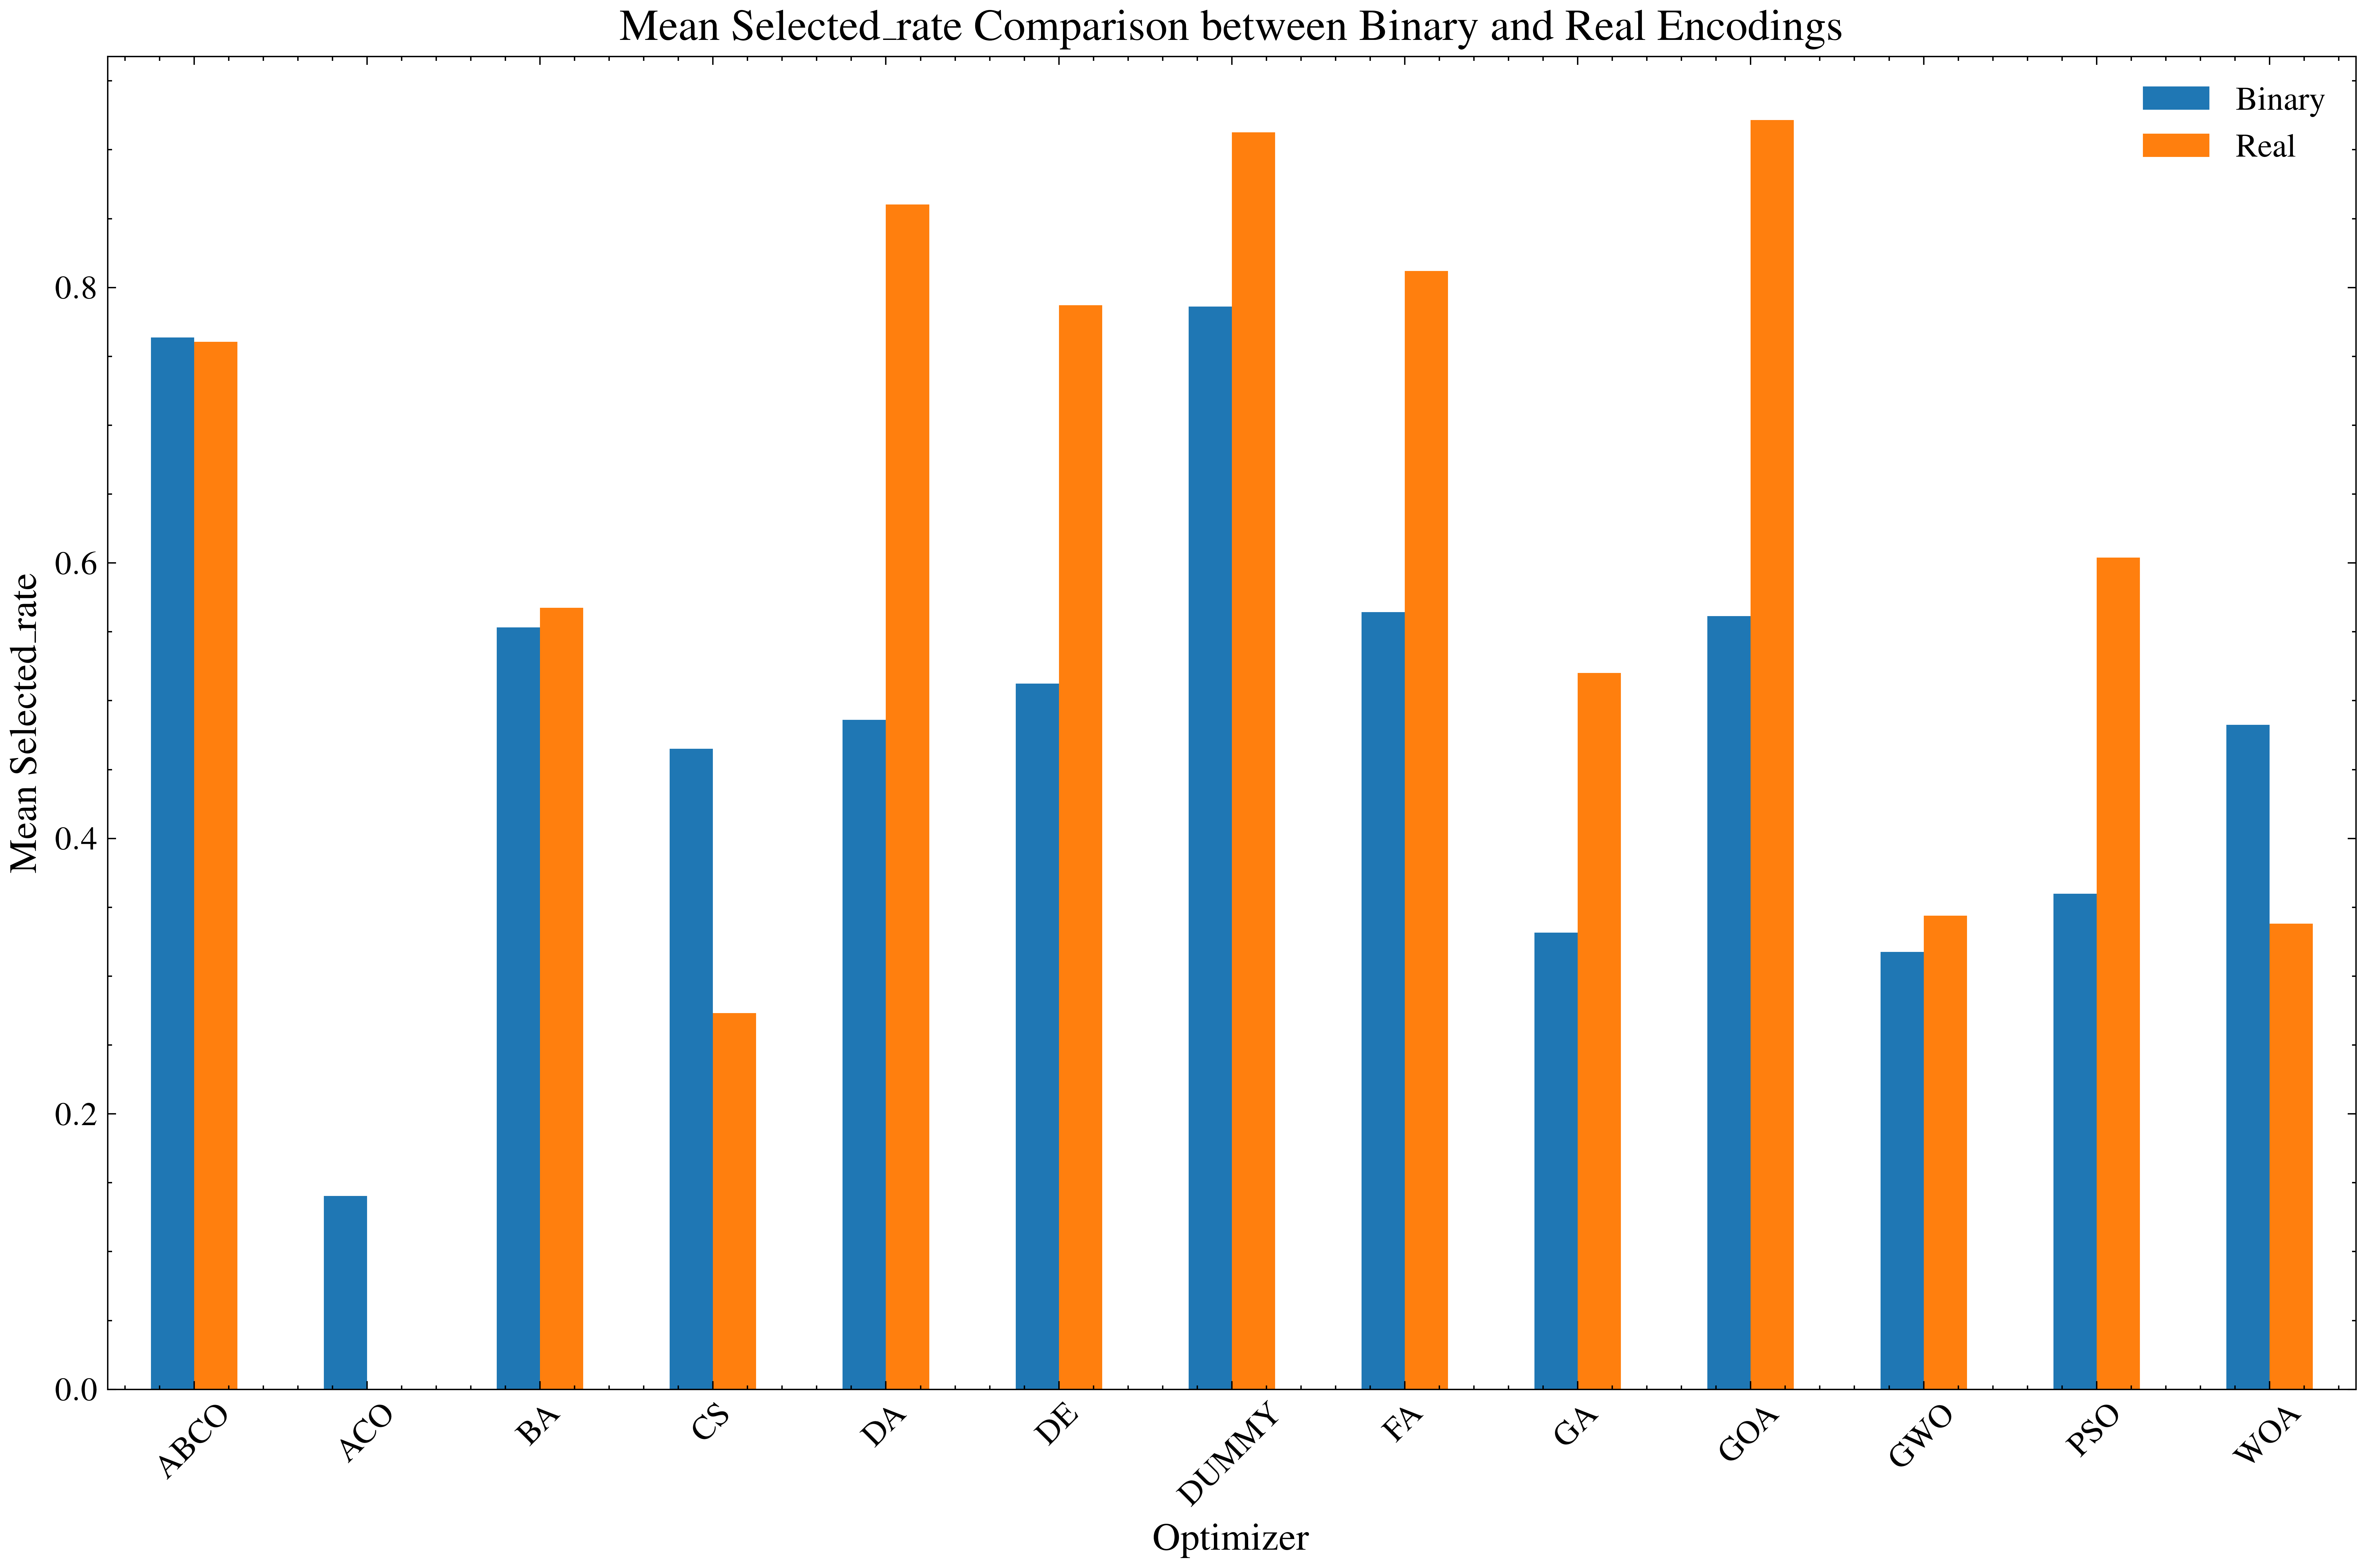
\includegraphics[width=1\textwidth]{imagenes/chapter6/selected_rate_comparison.png}
            \end{center}
            \caption{Comparación binaria vs continuo en selección de características}
        \end{figure}
        \column{0.5\textwidth}
        \begin{itemize}
            \item ¿Merece pues la pena el uso de algoritmos específicos para la selección de características o las versiones originales son totalmente capaces de reducir?
        \end{itemize}
    \end{columns}
\end{frame}

\begin{frame}
    \frametitle{Preguntas investigadas}
    \begin{figure}
        \begin{center}
            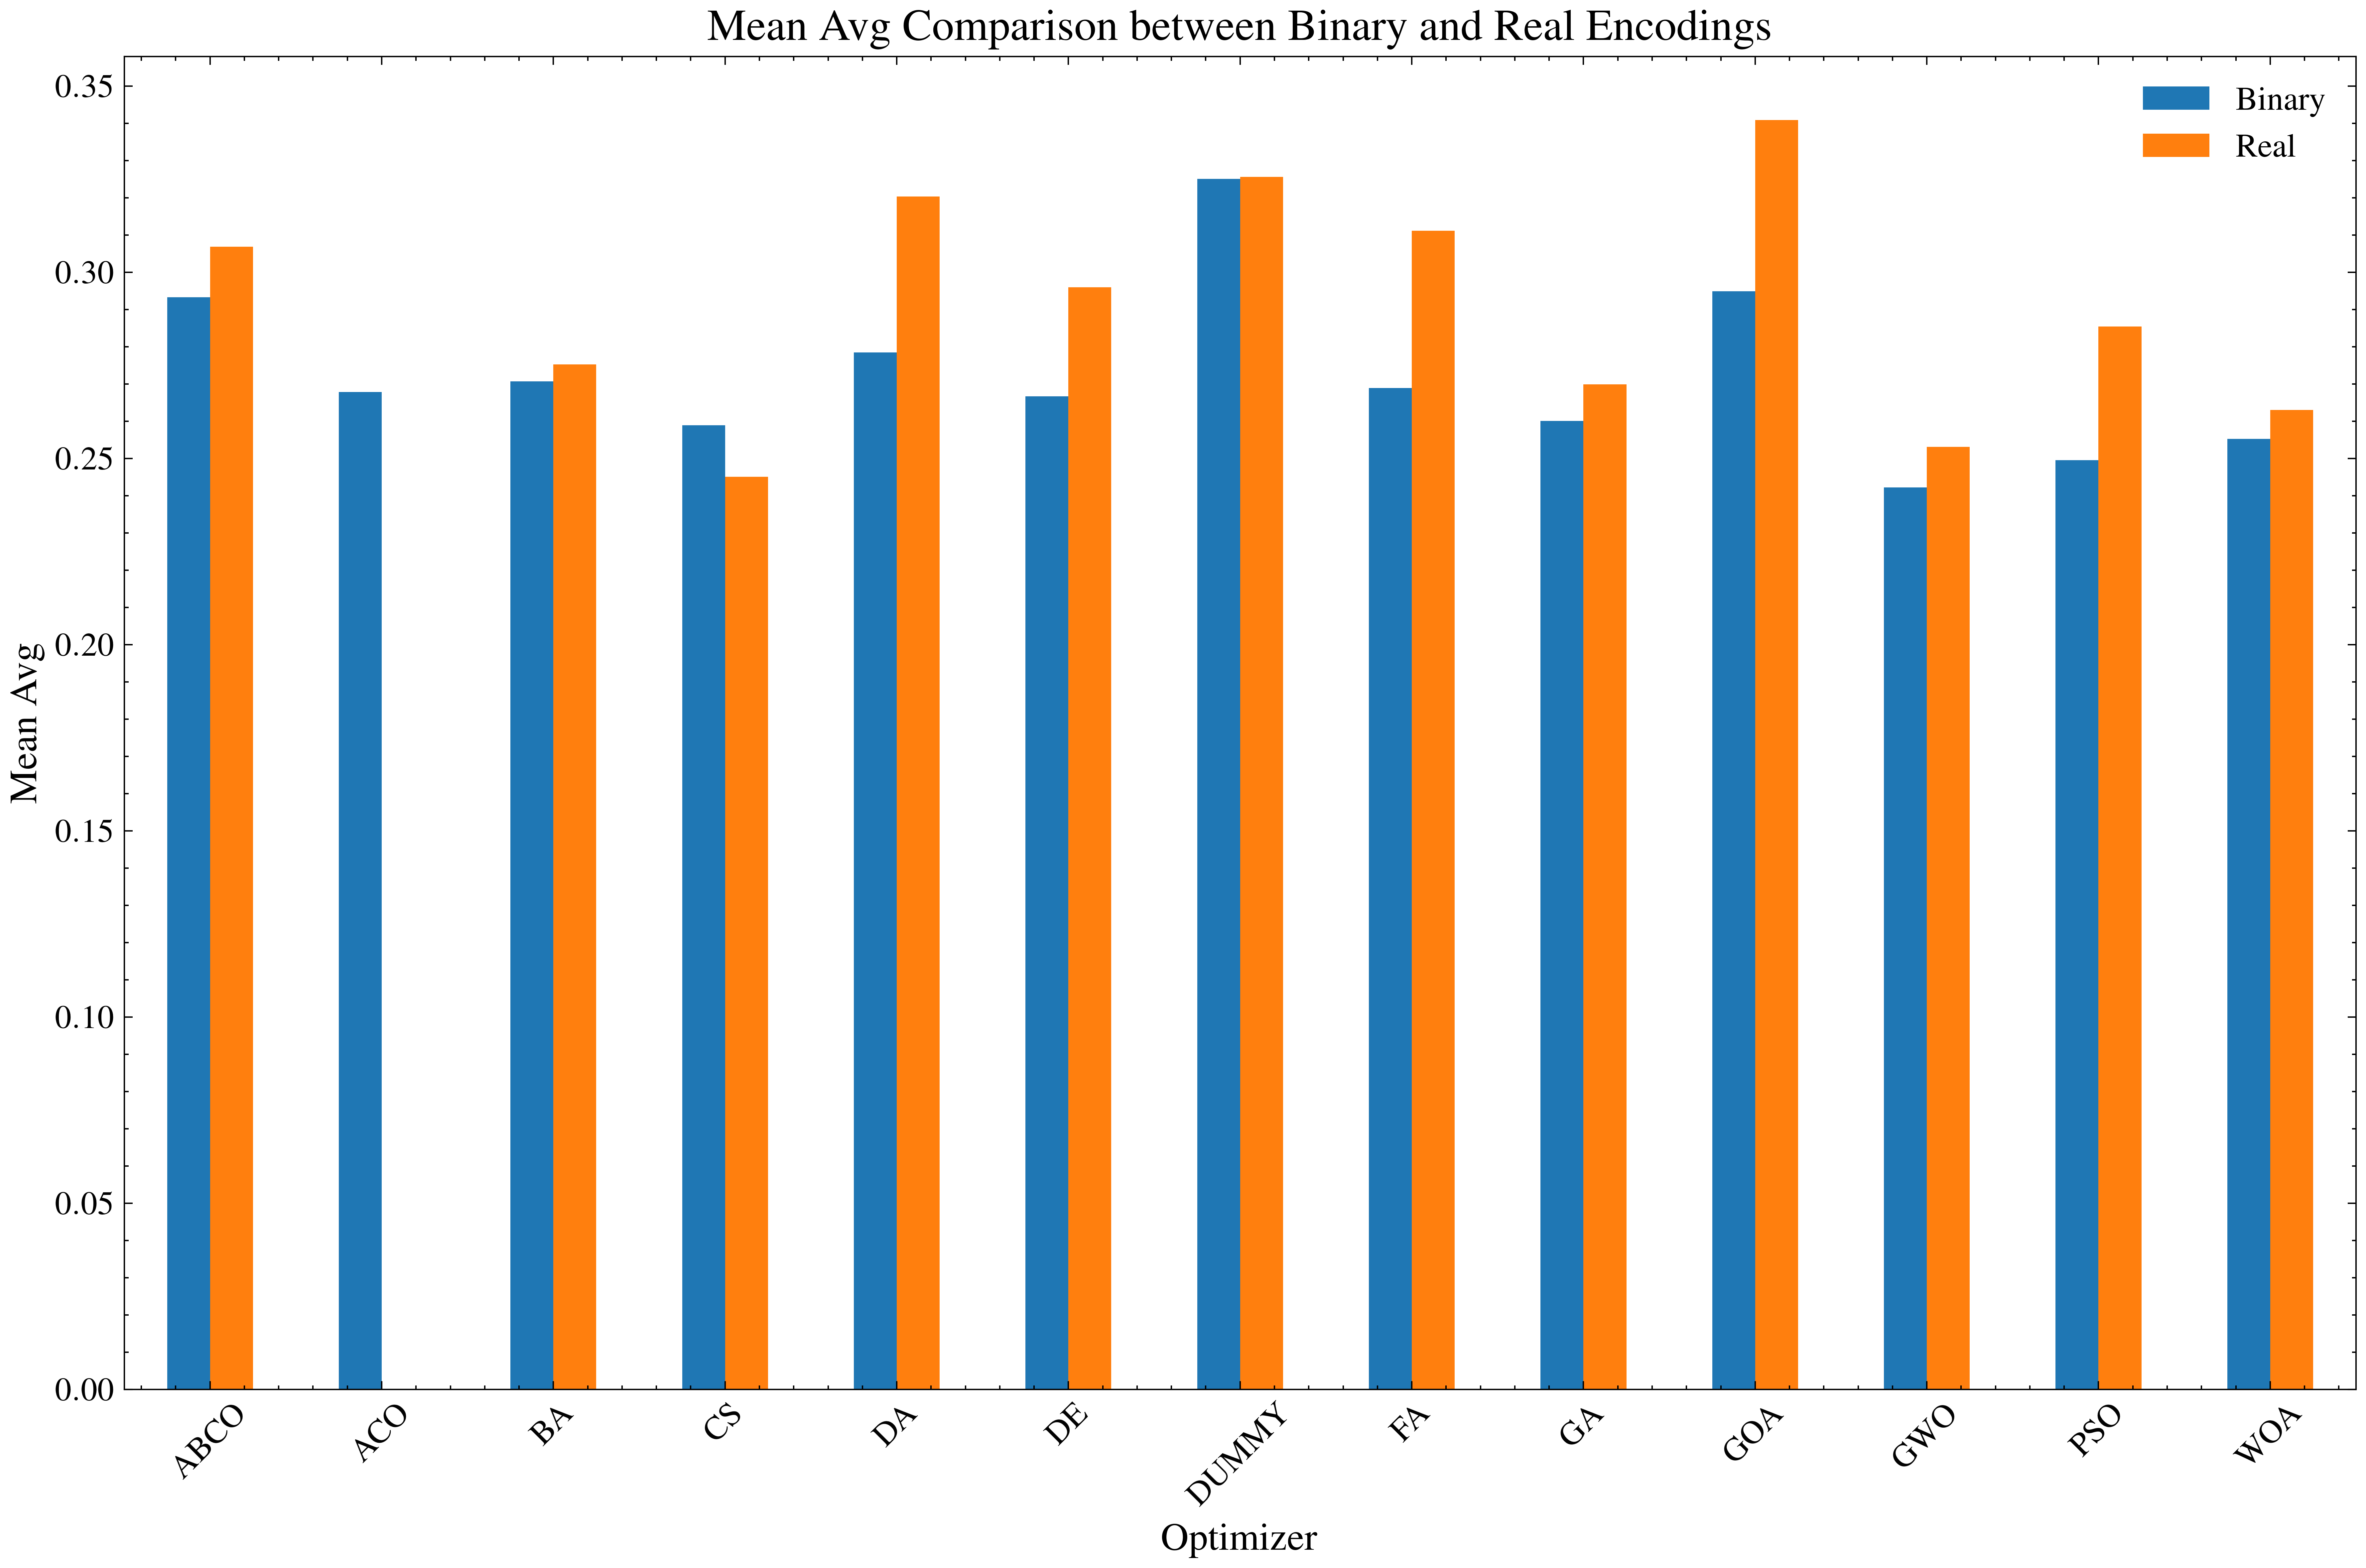
\includegraphics[width=0.6\textwidth]{imagenes/chapter6/avg_comparison.png}
        \end{center}
        \caption{Comparación de \textit{fitness} en binario vs continuo}
    \end{figure}
\end{frame}

\begin{frame}
    \frametitle{Preguntas investigadas}
    \begin{columns}
        \column{0.5\textwidth}
        \begin{itemize}
            \item ¿Cómo son los recientes en comparación con los más clásicos?
            \item ¿Cuáles de los recientes parecen más prometedores?
        \end{itemize}
        \column{0.5\textwidth}
        \begin{itemize}
            \item ¿Son los algoritmos buenos en su versión original igualmente eficaces en su versión binaria?
            \item ¿Cuáles son las opciones más interesantes dentro de ciertos contextos?
        \end{itemize}
    \end{columns}
\end{frame}